%%%% SIGNAL SECTION %%%%
\section{MCS Performance on Muons from numuCC Events in Simulation}\label{MC_performance_section}

\subsection{Input sample}
reference CCInclusive technote, good runs list, no EXT data used only BNB. cosmic backgrounds are low after event selection (quantify this probably).

\subsection{Event selection}
\begin{enumerate}
\item describe the event selection, 2 tracks at vertex, etc etc.
\item state we take tracks fully contained in fiducial volume, longer than 1 meter
\item in order to ensure good track reconstruction we match the track with an MCTrack by requiring the reco track starts and ends within 3cm of the MCTrack start and end.
\item with the MC sample used we ended up with 1613 such tracks.
\end{enumerate}

\subsection{MCS Energy Validation}\label{MCS_Energy_Validation_MCNuRecoTrack_section}
For this sample of reconstructed tracks, the trajectory points only of each track is used as input to the MCS code, described in Section XXX. The resulting MCS energy versus range-based energy without any additional hand-scan reconstruction quality checks can be seen in Figure \ref{MCS_range_energy_MCNuRecoTrack_noPDGcut_fig}. The off-diagonal visible in this figure (where MCS energy greatly overestimates range energy) is caused by MIDs, generally where the longest track is a proton. Figure \ref{MCS_range_energy_MCNuRecoTrack_withPDGcuts_fig} divides Figure \ref{MCS_range_energy_MCNuRecoTrack_noPDGcut_fig} into those events in which the MCTrack matched to the reconstructed track is a proton, a pion, or a muon. From this figure it is clear comparing MCS energy to range energy for contained tracks will provide a handle on separating muon tracks from proton tracks in data (though it is hard to make similar conclusions about pions due to limited statistics in this study).\\

In order to compute a bias and a resolution, Figure \ref{MCS_range_energy_MCNuRecoTrack_muononly_fig} is sliced in bins of range energy and a histogram of the fractional energy difference ($\frac{E_{MCS} - E_{range}}{E_{range}}$) is created for each bin. This distribution is shown for two representative bins in Figure \ref{MCS_range_bias_resolution_MCNuRecoTrack_slices_fig}. The mean of each distribution is used to compute a bias a function of range, while the standard deviation of each distribution is used to compute a resolution. The bias and resolution for this energy reconstruction method shown in Figure \ref{MCS_range_bias_resolution_MCNuRecoTrack_fig}. This figure indicates a bias in the MCS energy resolution on the order of a few percent, with a resolution that decreases from about 18\% for contained tracks with true total energy around 0.5 GeV (which corresponds to a length of about 1.7 meters) to below 10\% for contained tracks with true total energy greater than 0.8 GeV (which corresponds to a length of about 3.1 meters).


\begin{figure}[h!]
\begin{center}
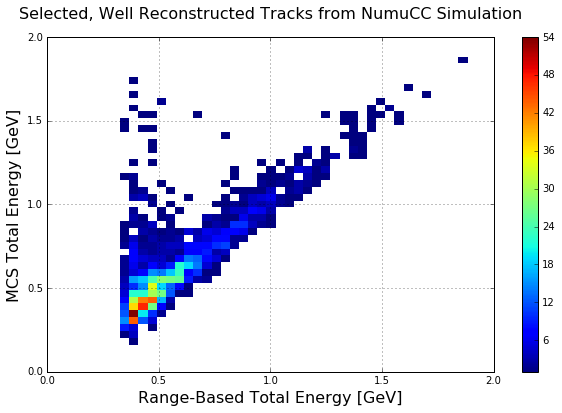
\includegraphics[width=100mm]{Figures/MCS_range_comparison_MCNuRecoTracks_noPDGcut.png}
\end{center}
\caption{\textit{MCS computed energy versus range energy for the selected simulated neutrino-induced fully contained, well reconstructed muon sample without any additional cuts to mitigate MIDs.}}
\label{MCS_range_energy_MCNuRecoTrack_noPDGcut_fig}
\end{figure}

\begin{figure}
\centering
\mbox{
	\subfigure[\textit{The subset of events in Figure \ref{MCS_range_energy_MCNuRecoTrack_noPDGcut_fig} in which the true identity of the track is a proton.}]
	{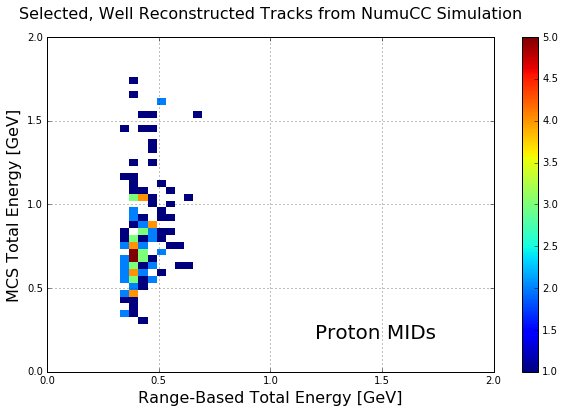
\includegraphics[width=50mm]{Figures/MCS_range_energy_MCNuRecoTracks_proton.png}}
	\quad
	\subfigure[\textit{The subset of events in Figure \ref{MCS_range_energy_MCNuRecoTrack_noPDGcut_fig} in which the true identity of the track is a pion.}]
	{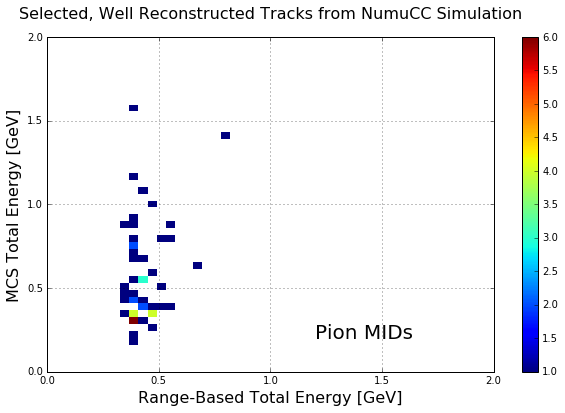
\includegraphics[width=50mm]{Figures/MCS_range_energy_MCNuRecoTracks_pion.png}}
	\quad
	\subfigure[\textit{The subset of events in Figure \ref{MCS_range_energy_MCNuRecoTrack_noPDGcut_fig} in which the true identity of the track is a muon.}\label{MCS_range_energy_MCNuRecoTrack_muononly_fig}]
	{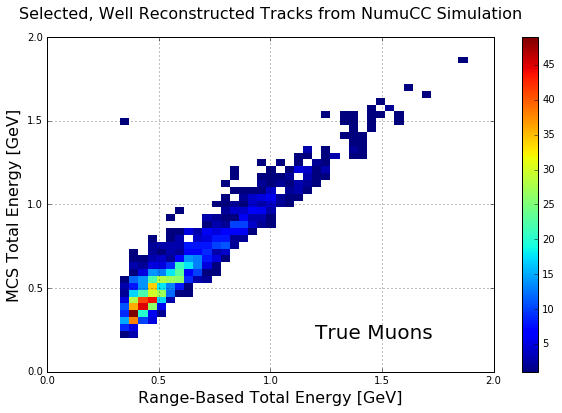
\includegraphics[width=50mm]{Figures/MCS_range_energy_MCNuRecoTracks_muon.png}}
	}
\caption{\textit{MCS computed energy versus range energy for the selected neutrino-induced, well reconstructed fully contained muon sample in simulation broken up by true particle identity of the track.}}
\label{MCS_range_energy_MCNuRecoTrack_withPDGcuts_fig}
\end{figure}


\begin{figure}
\centering
\mbox{
	\subfigure[\textit{Fractional energy difference between 0.35 and 0.53 GeV range energy.}]
	{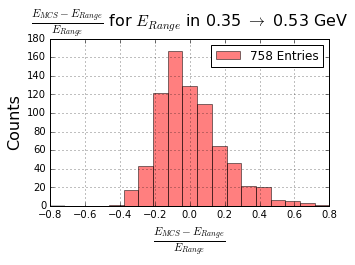
\includegraphics[width=50mm]{Figures/MCS_range_resolution_MCNuRecoTracks_slice1.png}}
	\quad
	\subfigure[\textit{Fractional energy difference between 0.90 and 1.08 GeV range energy.}]
	{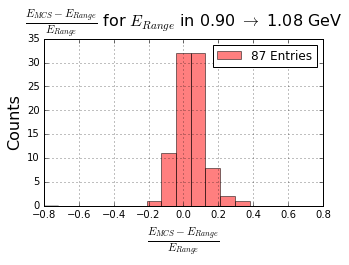
\includegraphics[width=50mm]{Figures/MCS_range_resolution_MCNuRecoTracks_slice2.png}}
	\quad
	\subfigure[\textit{Fractional energy difference between 1.45 and 1.63 GeV range energy.}]
	{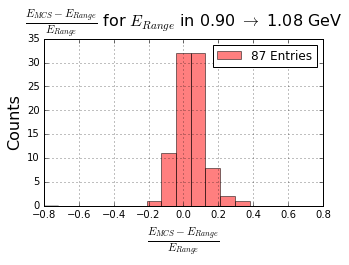
\includegraphics[width=50mm]{Figures/MCS_range_resolution_MCNuRecoTracks_slice2.png}}
	}

\caption{\textit{Fractional energy difference for a few representative bins of range energy derived from Figure \ref{MCS_range_energy_MCNuRecoTrack_muononly_fig}.}}
\label{MCS_range_bias_resolution_MCNuRecoTrack_slices_fig}
\end{figure}


\begin{figure}
\centering
\mbox{
	\subfigure[\textit{MCS energy bias as a function of range energy.}]
	{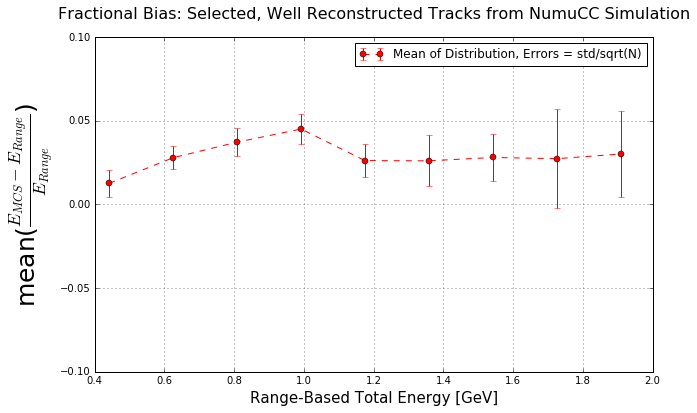
\includegraphics[width=75mm]{Figures/MCS_range_bias_MCNuRecoTracks.png}}
	\quad
	\subfigure[\textit{MCS energy resolution as a function of range energy.}]
	{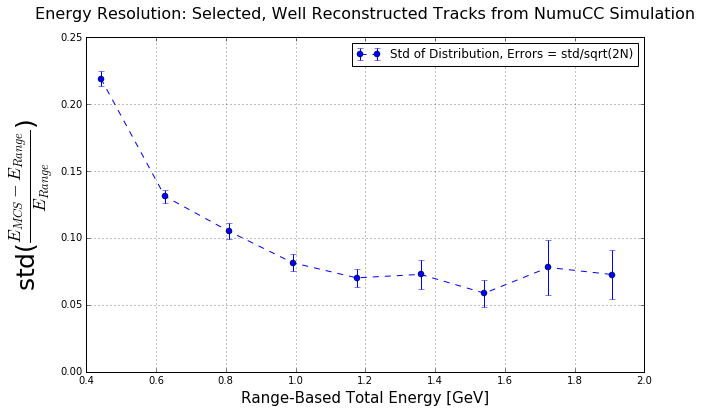
\includegraphics[width=75mm]{Figures/MCS_range_resolution_MCNuRecoTracks.png}}
	}
\caption{\textit{MCS energy bias and resolution as a function of range energy for the selected, well reconstructed neutrino-induced muons in {\ub} simulation.}}
\label{MCS_range_bias_resolution_MCNuRecoTrack_fig}
\end{figure}



\subsection{Highland Validation}\label{Highland_Validation_MCNuRecoTrack_section}
For a given track segment energy and length, 98\% of the angular scatter deviations should be gaussian with an RMS described by the Highland equation (Equation \ref{highland_eqtn}), while the remaining 2\% are larger angle Rutherford scatters [XXX source]. Therefore, a histogram of track segment angular deviations divided by the RMS predicted by the Highland equation should be gaussian with a width of unity. In this section, we validate this claim.\\

For each 20cm segment of each reconstructed track in this sample, the energy of the muon at the start of that segment is estimated by taking the computed MCS energy and subtracting out energy lost in the track upstream of the start of this segment, assuming the track was minimally ionizing (depositing 2.2 MeV per centimeter of track). This energy, along with the segment length, is converted into an expected RMS angular deviation by way of Equation \ref{highland_eqtn}. For each consecutive pairs of segments, the angular scatter in milliradians divided by the Highland expected RMS in millradians is an entry in the histogram shown in Figure \ref{Highland_validation_MCNuRecoTracks_fig}. From this figure we can see that the Highland formula is valid for well reconstructed tracks in data.

\begin{figure}[h!]
\begin{center}
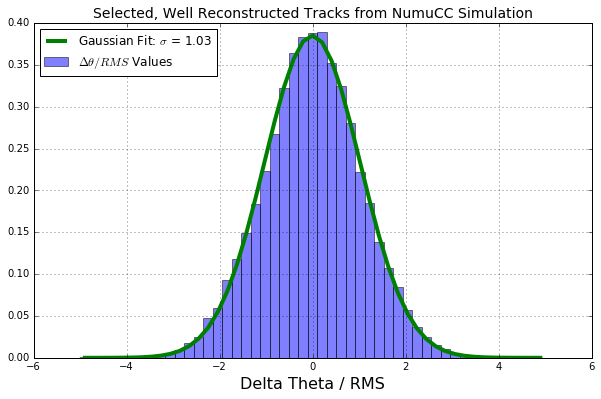
\includegraphics[width=100mm]{Figures/Highland_validation_MCNuRecoTracks_muon.png}
\end{center}
\caption{\textit{20cm segment angular deviations divided by expected Highland RMS for the sample of well reconstructed, neutrino induced muons in simulation.}}
\label{Highland_validation_MCNuRecoTracks_fig}
\end{figure}